%%%%%%%%%%%%%%%%%%%%%%%%%%%%%%%%%%%%%%%%%%%%%%%%%%%%%%%%%%%%%%%%%%%%%%%%
% Preamble
%%%%%%%%%%%%%%%%%%%%%%%%%%%%%%%%%%%%%%%%%%%%%%%%%%%%%%%%%%%%%%%%%%%%%%%%
\documentclass[11pt]{article}
%
% Packages and other includes
% Pagination
\usepackage[letterpaper, margin=1in]{geometry}
\usepackage{emptypage}
%
% Fonts
\usepackage[T1]{fontenc} % best for Western European languages
\usepackage{lmodern} % Latin Modern instead of CM
\usepackage{textcomp} % required to get special symbols
%
% Math
\usepackage{amsmath, amssymb}
\usepackage{braket}
%
% Graphics, floats, tables
\usepackage{graphicx, color, float, array}
%
% Hyperlinks
\usepackage{hyperref}
%
%
% Definitions and settings
% Paragraph indent and spacing
\setlength{\parskip}{0.4\baselineskip}
\setlength{\parindent}{0in}
%
%
% Title, authors, date
\title{\textbf{Final Review}}
\date{\vspace{-2em}March 12, 2022}
%
%
%%%%%%%%%%%%%%%%%%%%%%%%%%%%%%%%%%%%%%%%%%%%%%%%%%%%%%%%%%%%%%%%%%%%%%%%
% Main document
%%%%%%%%%%%%%%%%%%%%%%%%%%%%%%%%%%%%%%%%%%%%%%%%%%%%%%%%%%%%%%%%%%%%%%%%
%

\begin{document}

\maketitle

This is a checklist based on the lecture and textbook materials. It is not
expected to be an all encompassing study guide and provides a guideline for
your studies.

\begin{itemize}
\item[] \textbf{Phase Equilibria}
  \begin{center}
    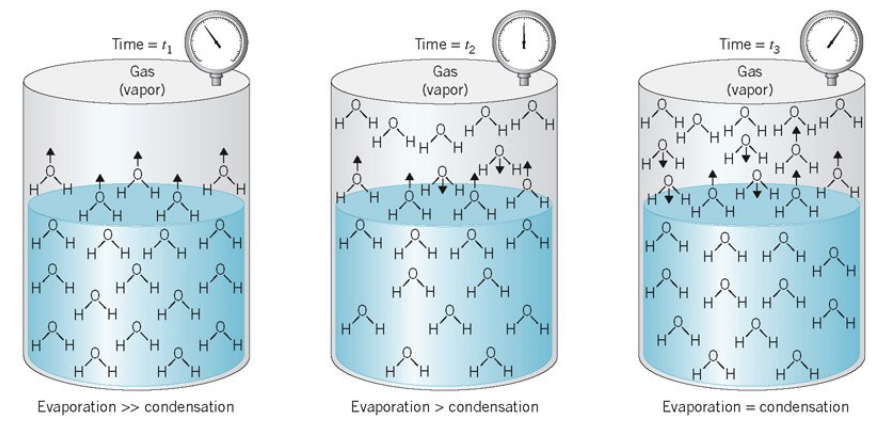
\includegraphics[scale=0.35]{vapor.png}
  \end{center}
\item Vapor pressure and boiling points
\item Trouton's rule ($\Delta S_\text{vap} = 85$ J/(mol K))
\item Clausius-Clapeyron equation
  \begin{align*}
    P_f = P_i e^{-\frac{\Delta H_\text{vap}}{R}(\frac{1}{T_f}-\frac{1}{T_i})}
  \end{align*}
\item[] \textbf{Phase Diagram}
\item Gibbs Phase Rule $F = C - P + 2$
\item Triple Point and Critical Point
  \begin{center}
    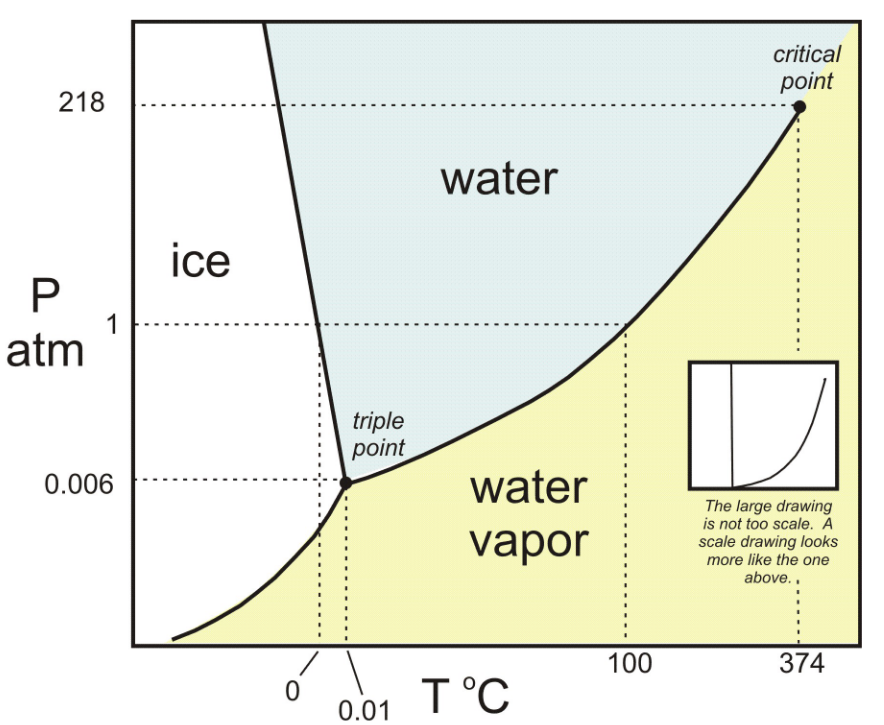
\includegraphics[scale=0.3]{water_phase.png}
  \end{center}
\item Kinetics of Phase Changes
\item Real Gases and the Van der Waals Equation
  \begin{align*}
    (P+\frac{a}{v^2})(v-b) = RT
  \end{align*}
\item Microscopic interpretation of constants $a$ and $b$
\item[] \textbf{Intermolecular Interactions}
\item Electrostatic, induction, and dispersion
\item Affects boiling points and vapor pressures
\item[] \textbf{Solutions}
\item ``Like dissolves like''
\item Molarity (mol/L), molality (mol/kg), mass percentage ($m$(solute)/$m$(solution)),
  and mole fraction ($\chi = \frac{n(\text{solute})}{n(\text{solution})}$)
\item Solubility rules for ionic compounds
\item Henry's law $c(\text{solute}) = k_HP(\text{solute})$
\item Temperature dependence of solubility
  \begin{center}
    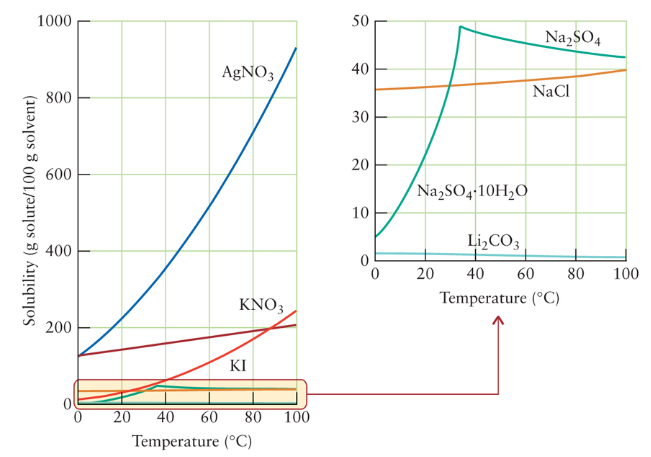
\includegraphics[scale=0.5]{solubility.png}
  \end{center}
\item Raoult's law
  \begin{align*}
    \Delta P = P(\text{sol}) - P_0 = -\chi(\text{solute})P_0(\text{solvent})
  \end{align*}
\item Boiling point elevation ($\Delta T_\text{bp} = k_b b$) and freezing
  point depression ($\Delta T_\text{fp} = -k_fb$)
\item Osmotic pressure ($\Pi$) satisfies ``ideal gas law''
  \begin{center}
    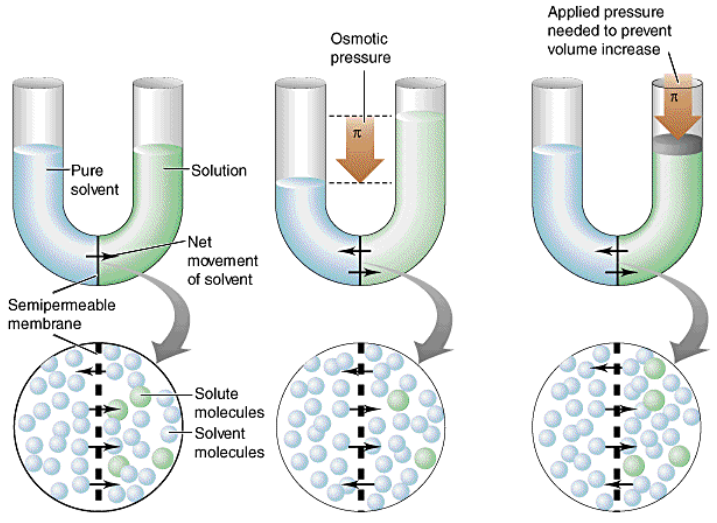
\includegraphics[scale=0.4]{osmotic.png}
  \end{center}
\item Van't Hoff factor multipled to freezing point depression and
  boiling point elevation
  \begin{align*}
    i=\frac{n(\text{solute species in solution})}
    {n(\text{undissociated solute})}
  \end{align*}
\item Osmotic pressure: $\Pi V = inRT$
\item[] \textbf{Solids}
\item Unit cell is smallest unit that can be used to
  construct the lattice by periodic repetition
\item Lattice points: Atomic coordinates in basis
  of lattice vectors \textbf{a, b, c}
  \begin{center}
    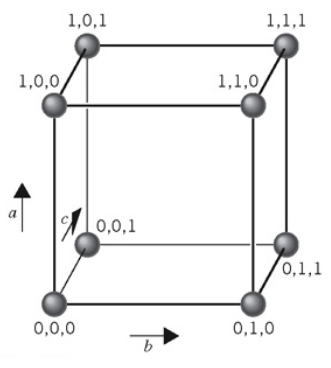
\includegraphics[scale=0.4]{solids.png}
  \end{center}
\item $N_u$ - number of atoms per unit cell; $V_u$ unit cell volume
\item Density where $m = M/N_A$ is atomic mass
  \begin{align*}
    \rho = \frac{m_u}{V_u} = \frac{N_um}{V_u}
  \end{align*}
\item Different packings - simple cubic, body-centered cubic, and face-centered cubic
\end{itemize}

\end{document}
